\section{Motivation and first Examples}
Quantum mechanics is the physical theory that describes elementary processes on the microscopic level. In this chapter we will touch the essential aspects of the theory from a quantum algorithmic perspective. At the end we will construct a small, but famous, quantum algorithm -- the \texttt{Deutsch} algorithm. Although it isn't very useful in practice, it is an excellent example that illustrates many important aspects of quantum mechanics in general, and quantum algorithmics especially.\\

Imagine an experiment with an elementary particle (e.g. an Electron or a Photon) which we can observe in two states labeled as $\ket{0}$ and $\ket{1}$. This could be the magnetic moment (``spin'') of the electron or the polarization of the photon. In the first case, you can imagine the observation of the spins allignment to be performed by switching on an external magnetic field, the field will then either increase or decrease a tiny bit (depending if the magnetic moment of the electron points in the same direction of the external or opposite). You can also imagine something more illustrative, like a coin that can be either heads or tails, or a marble in a double half-pipe or ``double-well''
\begin{align*}
    \ket{0}\equiv\raisebox{-0.9cm}{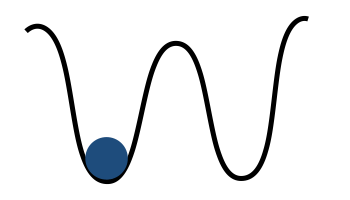
\includegraphics[width=0.25\textwidth]{src/doublewell-left.png}},\quad
    \lvert 1 \rangle \equiv \raisebox{-0.9cm}{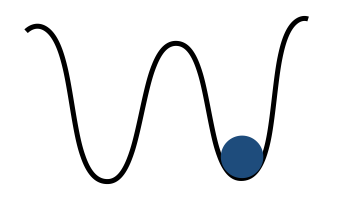
\includegraphics[width=0.25\textwidth]{src/doublewell-right.png}}
\end{align*}
that has two localized states: ``left'' and ``right'', which we just call the state $\lvert 0\rangle$ and $\lvert 1\rangle$.
For all examples given, we can just label the two states as 0 and 1 -- the $\ket{}$ notation is used to denote that $\ket{a}$ is the state that we labelled with the symbol $a$ (it is just more convenient than subscripts).\\
Classical realization of such binary systems are called \textit{bits}, while we call the quantum versions \textit{qubits}. A qubit, an idealized quantum two-state system, is therefore the quantum version of a bit, an idealized classical two-state system. \\

Now consider a ``coin-flip'' process $U$ that \textit{acts} on the \textit{state} of our particle.  If we observe the particle afterwards we can either find it in state $\ket{0}$ with probabilty $p_0 = \frac{1}{2}$ and in state $\ket{1}$ with probability $p_1 = \frac{1}{2}$ -- for both possible input states.\\

For the examples with elementary particles, you can imagine it like a black-box which the particle ``flies'' through and some physical interactions happen inside the box.
For our ``double-well'' example above, this process is basically placing the marble at the center where it will eventually fall down the right or left side (with a sufficient symmetric double-well potential, the probabilities will be fifty-fifty)

\begin{align*}
    \raisebox{-0.9cm}{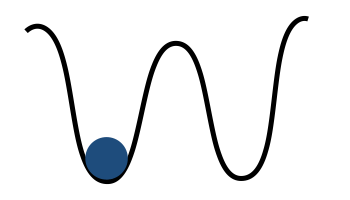
\includegraphics[width=0.25\textwidth]{src/doublewell-left.png}} \leftarrow \raisebox{-0.9cm}{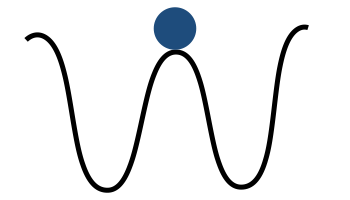
\includegraphics[width=0.25\textwidth]{src/doublewell-center.png}} \rightarrow \raisebox{-0.9cm}{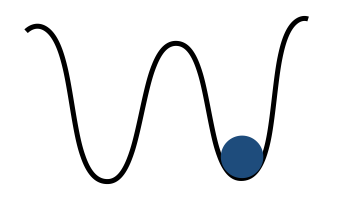
\includegraphics[width=0.25\textwidth]{src/doublewell-right.png}}.
\end{align*}
However, we are not aiming to find an exact mechanical description (how to realize the process for an explicit physical system), but rather a general description about the outcome of the process (ignoring the mechanical realization).


\subsection*{A Classical Probabilistic Process (Coin Flips)}
Let's describe the process $U$ as a classical process. To emphasize it, we will label it as $U_\text{C}$.
An obvious candidate that comes to mind is the description of $U_\text{C}$ as a probabilistic process that ``flips'' the particle with 50\% probability. The process takes the state $\ket{k}$ with $k \in [0,1]$ as an input and outputs $\ket{k\oplus 1}$\footnote{$\oplus$ denotes logical addition $k\oplus l = \left(k+l\right)\mod2$. Explicitly: $0\oplus0=0, 0\oplus1=1\oplus0=1, 1\oplus1=0$. The function $f(x) = x \oplus 1$ on bit value $x$ is for example the same as a logical \textsc{not} operation.} with 50\% probability. We could write it as
\begin{align}
    \ket{i} \xrightarrow{U_\text{C}}  \begin{cases} \ket{i} \text{ with } p=1/2 \\ \ket{i\oplus 1} \text{ with } \tilde{p}=1-p \end{cases}.
\end{align}
Now suppose a new process $U_\text{C}^2$ that executes the original process $U_\text{C}$ twice
\begin{align}
    \ket{k} \xrightarrow{U_\text{C}}  \xrightarrow{U_\text{C}} \ket{l}.
\end{align}

The end result $\ket{l}$ will either be $l=0$ or $l=1$ with probabilities of 50\%. We can see this by looking at the probabilities of all individual outcomes of the $U^2_\text{C}$ process
\begin{align}
      \ket{i} \xrightarrow{U_\text{C}} \begin{cases} \ket{i}\phantom{\oplus 0}
      \xrightarrow{U_\text{C}}
      \begin{cases} \ket{i}\phantom{\oplus 0}  \\ \ket{i \oplus 1} \end{cases} \\ \ket{i \oplus 1} \xrightarrow{U_\text{C}} \begin{cases} \ket{i\oplus 1} \\ \ket{i \oplus 1 \oplus 1} =\ket{i} \end{cases}  \end{cases}.  
\end{align}
The probabilitiy for each individual outcome is the product of the probabilities of the two individual processes $0.5\cdot 0.5 = 0.25$ and as $1\oplus 1 = 0$ we have only two different outputs of $U^2_\text{C}$, the two bit values $\ket{0}$ and $\ket{1}$ each with accumulated probability $0.5$. Our description of the given process as a probabilistic bit-flip with $p=0.5$ in series is therefore \textit{idempotent} which means $U_\text{C}^2 = U_\text{C}$.

\subsection{Quantum Process}

Another way that seems more complicated on first glance, is to allow \textit{superpositions}~\footnote{basically another word for \textit{linear combination}} of the states $\ket{0}$ and $\ket{1}$
\begin{align}
    \ket{\psi} = c_0\ket{0} + c_1\ket{1},\quad c_0,c_1\in \mathbb{C},
\end{align}
with the interpretation that the probability to observe the particle in $\ket{i}$ is given by $p_i = |c_i|^2$ for $i\in\left\{0,1\right\}$. We call the coefficients $c_i$ the \textit{probability amplitutes} for the \textit{basis state} $\ket{i}$. 
To ensure consistency with this probability interpretation, we need to enforce a normalization condition on the amplitudes
\begin{align}
    |c_0 |^2 + | c_1 |^2 = 1. 
\end{align}
The action of our process, in the quantum version denoted as $\hd$, is assumed to act \textit{linear} on such a superposition
\begin{align}
    \hd\ket{\psi} = c_0 \hd\ket{0} + c_1 \hd\ket{1}.
\end{align}

In order to describe our process, we can now define the action of $\hd$ on the two basis states as
\begin{align}
    \hd\ket{0} &= \frac{1}{\sqrt{2}}\left( \ket{0} + \ket{1} \right) \equiv \ket{+}, \\
    \hd\ket{1} &= \frac{1}{\sqrt{2}}\left( \ket{0} - \ket{1} \right) \equiv \ket{-}.\label{eq:U|1>}
\end{align}
At this point one might ask why the minus sign and the $\frac{1}{\sqrt{2}}$ factor enter the equations. Both have to do with the interpretability of the coefficients in the linear combinations as probability amplitudes. We have abbreviated the positive and negative superposition of the two basis states as $\ket{\pm}$, as we will encounter them again in later chapters. \\

At this point, the observable outcome of the process $\hd$ on the states $\ket{0}$ and $\ket{1}$ is the same as before: 50\% observed in the unchanged input state $\ket{k}$, and 50\% observed in the flipped state $\ket{k\oplus 1}$. 
If we however investigate the outcomes of $U^2$ the results change with respect to our classical description
\begin{align}
    \hd^2\ket{k} &= \frac{1}{\sqrt{2}} \hd \left( \ket{0} + (-1)^k \ket{1} \right),\\
    &= \frac{1}{2} \left( \ket{0} + \ket{1} + (-1)^k \ket{0} - (-1)^k \ket{1} \right),\\
    &= \frac{1}{2} \left( (1+(-1)^k)\ket{0} + (1 + (-1)^{k+1})\ket{1} \right)\label{eq:U2|k>}
\end{align}
or, with explicit values for the two choices of the input state $\ket{k}$:
\begin{align}
    \hd^2\ket{k} = \begin{cases}
        \ket{0} \text{ if } k=0 \\
        \ket{1} \text{ if } k=1
    \end{cases}
\end{align}
so that we can write
\begin{align}
    \hd^2\ket{k} = \ket{k}
\end{align}
meaning we will always observe the unchanged input state after the process $\hd^2$ -- the process $\hd$ is \textit{self-inverse} (or \textit{involutory)}. This differs from our classical process $U_\text{C}^2$! The reason for this is the negative probability amplitude introduced in Eq.~\eqref{eq:U|1>} that leads to \textit{destructive interference} of the amplitudes in Eq.~\eqref{eq:U2|k>}. Although this is fundamentally different behaviour compared to our classical probabilistic description before, such interference phenomena are also common in ``classical'' macroscopic systems. The typical example are waves (e.g. water-waves, sonic-waves). The states $\ket{\psi}$ are therefore often called \textit{wavefunctions}.\\

The $\hd$ operation is called Hadamard operation -- it's origin is not in quantum mechanics. 

\subsection*{Path Sum Representation}
We can represent the quantum process above as so-called path-sums~\footnote{the more widespread term is path integral, but here we are discrete so we have a path sum}.
To illustrate the concept, let us first start with the classical probabilistic process, where Eq.~\eqref{eq:probabilistic-path-sum-1} is already given as a path sum. We start with our initial classical state (e.g. $\ket{0}$) as a node, a deterministic step will be represented by an arrow to the next state (e.g. a classical \texttt{not} would be $\ket{i} \rightarrow \ket{i\oplus 1}$), which a probabilistic step will be reprented by multiple arrows pointing to different new states. The arrows are then labelled with the corresponding probability.
For the process $\mathcal{P}^{1/2}_{\oplus}\mathcal{P}^{1/2}_{\oplus}$ this would look like
\begin{align}
    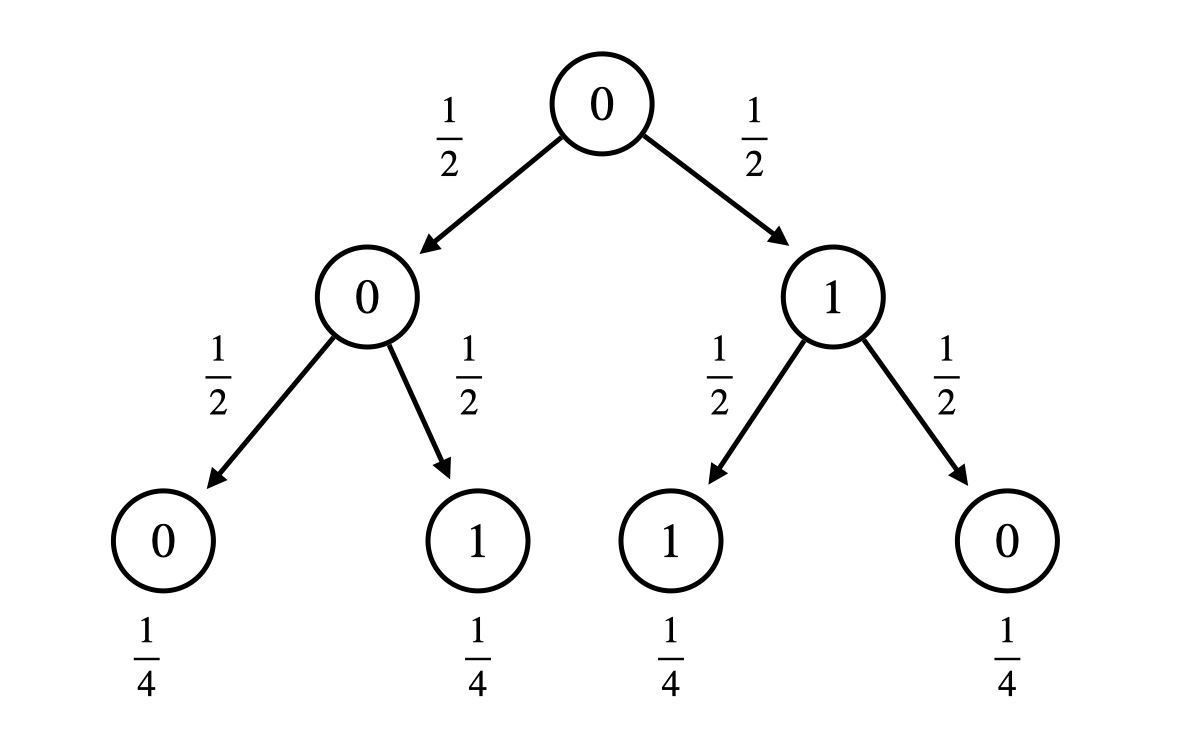
\includegraphics[width=0.5\textwidth]{src/ps_classical.jpeg}
\end{align}
where the numbers on the bottom line denote the total probability to end up in one of the four possible paths. The total probability assigned to each of the leaves in this binary tree is simply computed by walking the path from the root to the leaf and multiplying all probabilities on the way. To calculate the total probability to end up in one of the possible states (i.e. the bit is in 0 or 1) we just sum up the path probabilities that end up in the corresponding states -- therefore the name ``path sum''.\\
For the quantum process we can essentially create the sam path sum representation with just a slight change: now we use probability amplitudes instead of probabilities
\begin{align}
    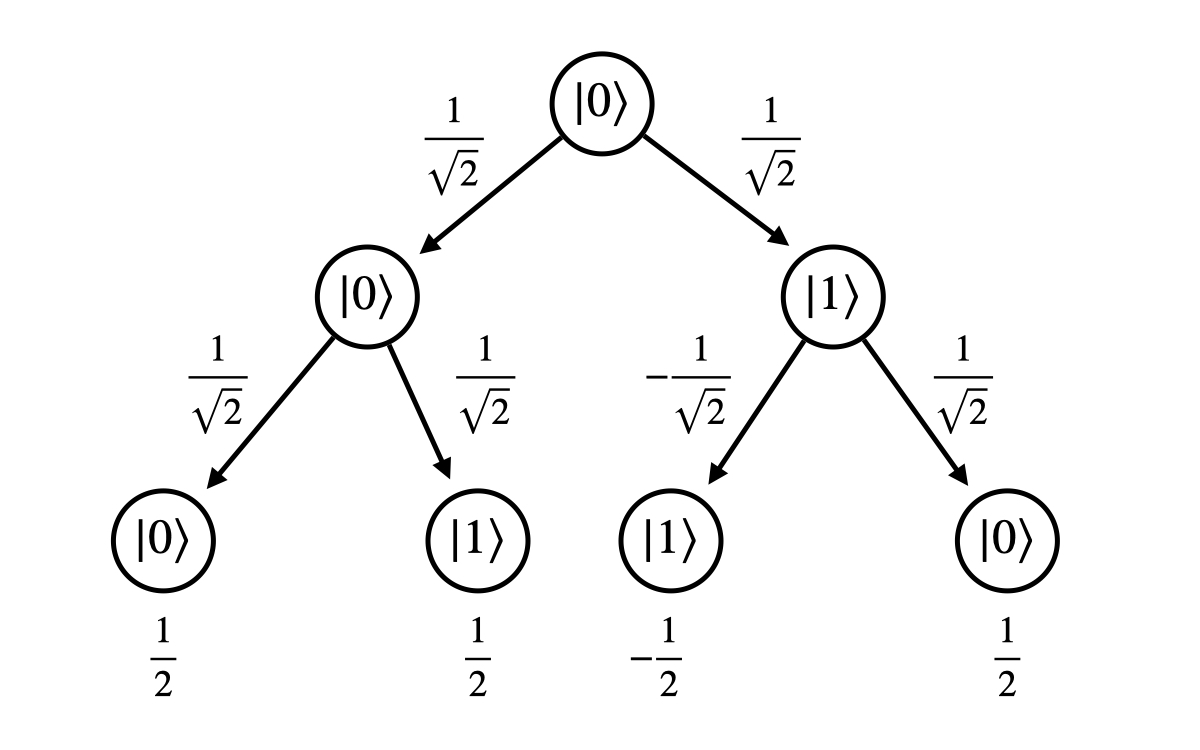
\includegraphics[width=0.5\textwidth]{src/ps_quantum.jpeg}
\end{align}
Now the numbers denoted under the leaves are the accumulated probability amplitudes (or short: path amplitudes) for the corresponding paths which are computed in the same manner, but simply multiplying all probability amplitudes on the corresponding path. 
The total probability amplitude for each of the states $\ket
{0}$ and $\ket{1}$ is then given by the sum of all path amplitudes with paths leading to the corresponding state. In this case, the total amplitude for $\ket{1}$ is $1/2 - 1/2 = 0$ so the state $\ket{1}$ will never be observed after the process.

\subsection{A First Quantum Algorithm}

\begin{def*}
\noindent\textbf{Deutsch Problem:} Take a Boolean function $f$ acting on a single bit. Determine if $f$ is constant, \textit{i.e.} if $f(0)=f(1)$.
\end{def*}

\begin{algo*}
\noindent\textbf{Classical Algorithm:} The algorithm is simple. We evaluate $f(0)$ and $f(1)$ and compare the results. In terms of oracle-complexity or ``query-complexity'' (``how often do we need to query the function $f$'') this needs two calls to $f$ (in all cases).
\end{algo*}

\paragraph{Quantum Algorithm:} 
The quantum algorithm is a bit more complex, but it manages to get away with a \textit{single call} to a quantum operation that contains the function $f$.\\
First, we need to define this quantum operation which shall act on the ``(computational) basis states'' (the quantum states that correspond to the classical bit states) as
\begin{def*}[Deutsch oracle]
\begin{align}
    U_f \ket{k} = (-1)^{f(k)} \ket{k}, \quad k \in \left\{0,1\right\}.
\end{align}
\end{def*}
This is a so-called ``phase-encoding'' which encodes the Boolean function $f$ that maps to $\left\{0,1\right\}$ into the values $\left\{+1,-1\right\}$ called``phases''.~\footnote{``phases'' can be general complex numbers on the unit circle, \textit{i.e.} all numbers $e^{-i\varphi }$ with $\varphi \in \mathbb{R}$. Of course the numbers $\pm 1$ are included. Sometimes the number $\varphi$ is also called phase.} 
Having defined the Deutsch oracle, the actual algorithm is almost complete
\begin{algo*}[\texttt{Deutsch} algorithm]
The Deutsch algorithm solves the Deutsch problem with a single query to the oracle $U_f$. The algorithm is the sequence of operations $\hd U_f \hd$ applied to a qubit in state $\ket{0}$.
\begin{align}
    U_D \ket{0} = \hd U_f \hd \ket{0} = \begin{cases}
        \pm\ket{0}, & f\text{ is constant}\\
        \pm\ket{1}, & \text{else}.
    \end{cases}
\end{align}
If $f$ is constant we have 100\% chance of reading out $\ket{0}$ while otherwise we will always read out $\ket{1}$.
\end{algo*}
Let's see how the algorithm works, by walking through the individual steps
\begin{align}
    U_D \ket{0} &= \hd U_f \hd \ket{0} = \hd U_f \ket{+}\nonumber\\
    &= \hd \frac{1}{\sqrt{2}}\left(U_f\ket{0} + U_f\ket{1} \right) \nonumber\\
    &= \hd \frac{1}{\sqrt{2}} \left((-1)^{f(0)}\ket{0} + (-1)^{f(1)}\ket{1}\right).
\end{align}
At this point, it makes sense to inspect the four possible cases.\\

\textit{case 1: $f(0)=f(1)=0$ (constant 0)} 
\begin{align}
    \hd \frac{1}{\sqrt{2}} \left((-1)^{f(0)}\ket{0} + (-1)^{f(1)}\ket{1}\right) = \hd \ket{+} = \ket{0}
\end{align}
\textit{case 2: $f(0)=f(1)=0$ (constant 1)} 
\begin{align}
    \hd \frac{1}{\sqrt{2}} \left((-1)^{f(0)}\ket{0} + (-1)^{f(1)}\ket{1}\right) = -\hd \ket{+} = -\ket{0}
\end{align}
note that we can ``pull'' the ``global minus'' sign to the front (this is just basic arithmetics).\\
\textit{case 3: $f(k)=k$ ($f$ is unit operation)} 
\begin{align}
    \hd \frac{1}{\sqrt{2}} \left((-1)^{f(0)}\ket{0} + (-1)^{f(1)}\ket{1}\right) = \hd \ket{-} = \ket{1}
\end{align}
\textit{case 4: $f(k)=\neg k$ ($f$ is negation)} 
\begin{align}
    \hd \frac{1}{\sqrt{2}} \left((-1)^{f(0)}\ket{0} + (-1)^{f(1)}\ket{1}\right) = -\hd \ket{-} = -\ket{1}
\end{align}
Note that the signs do not change the probability of reading out $\ket{0}$ or $\ket{1}$. 

In the same way as before, we can construct a path-sum representation
\begin{align*}
   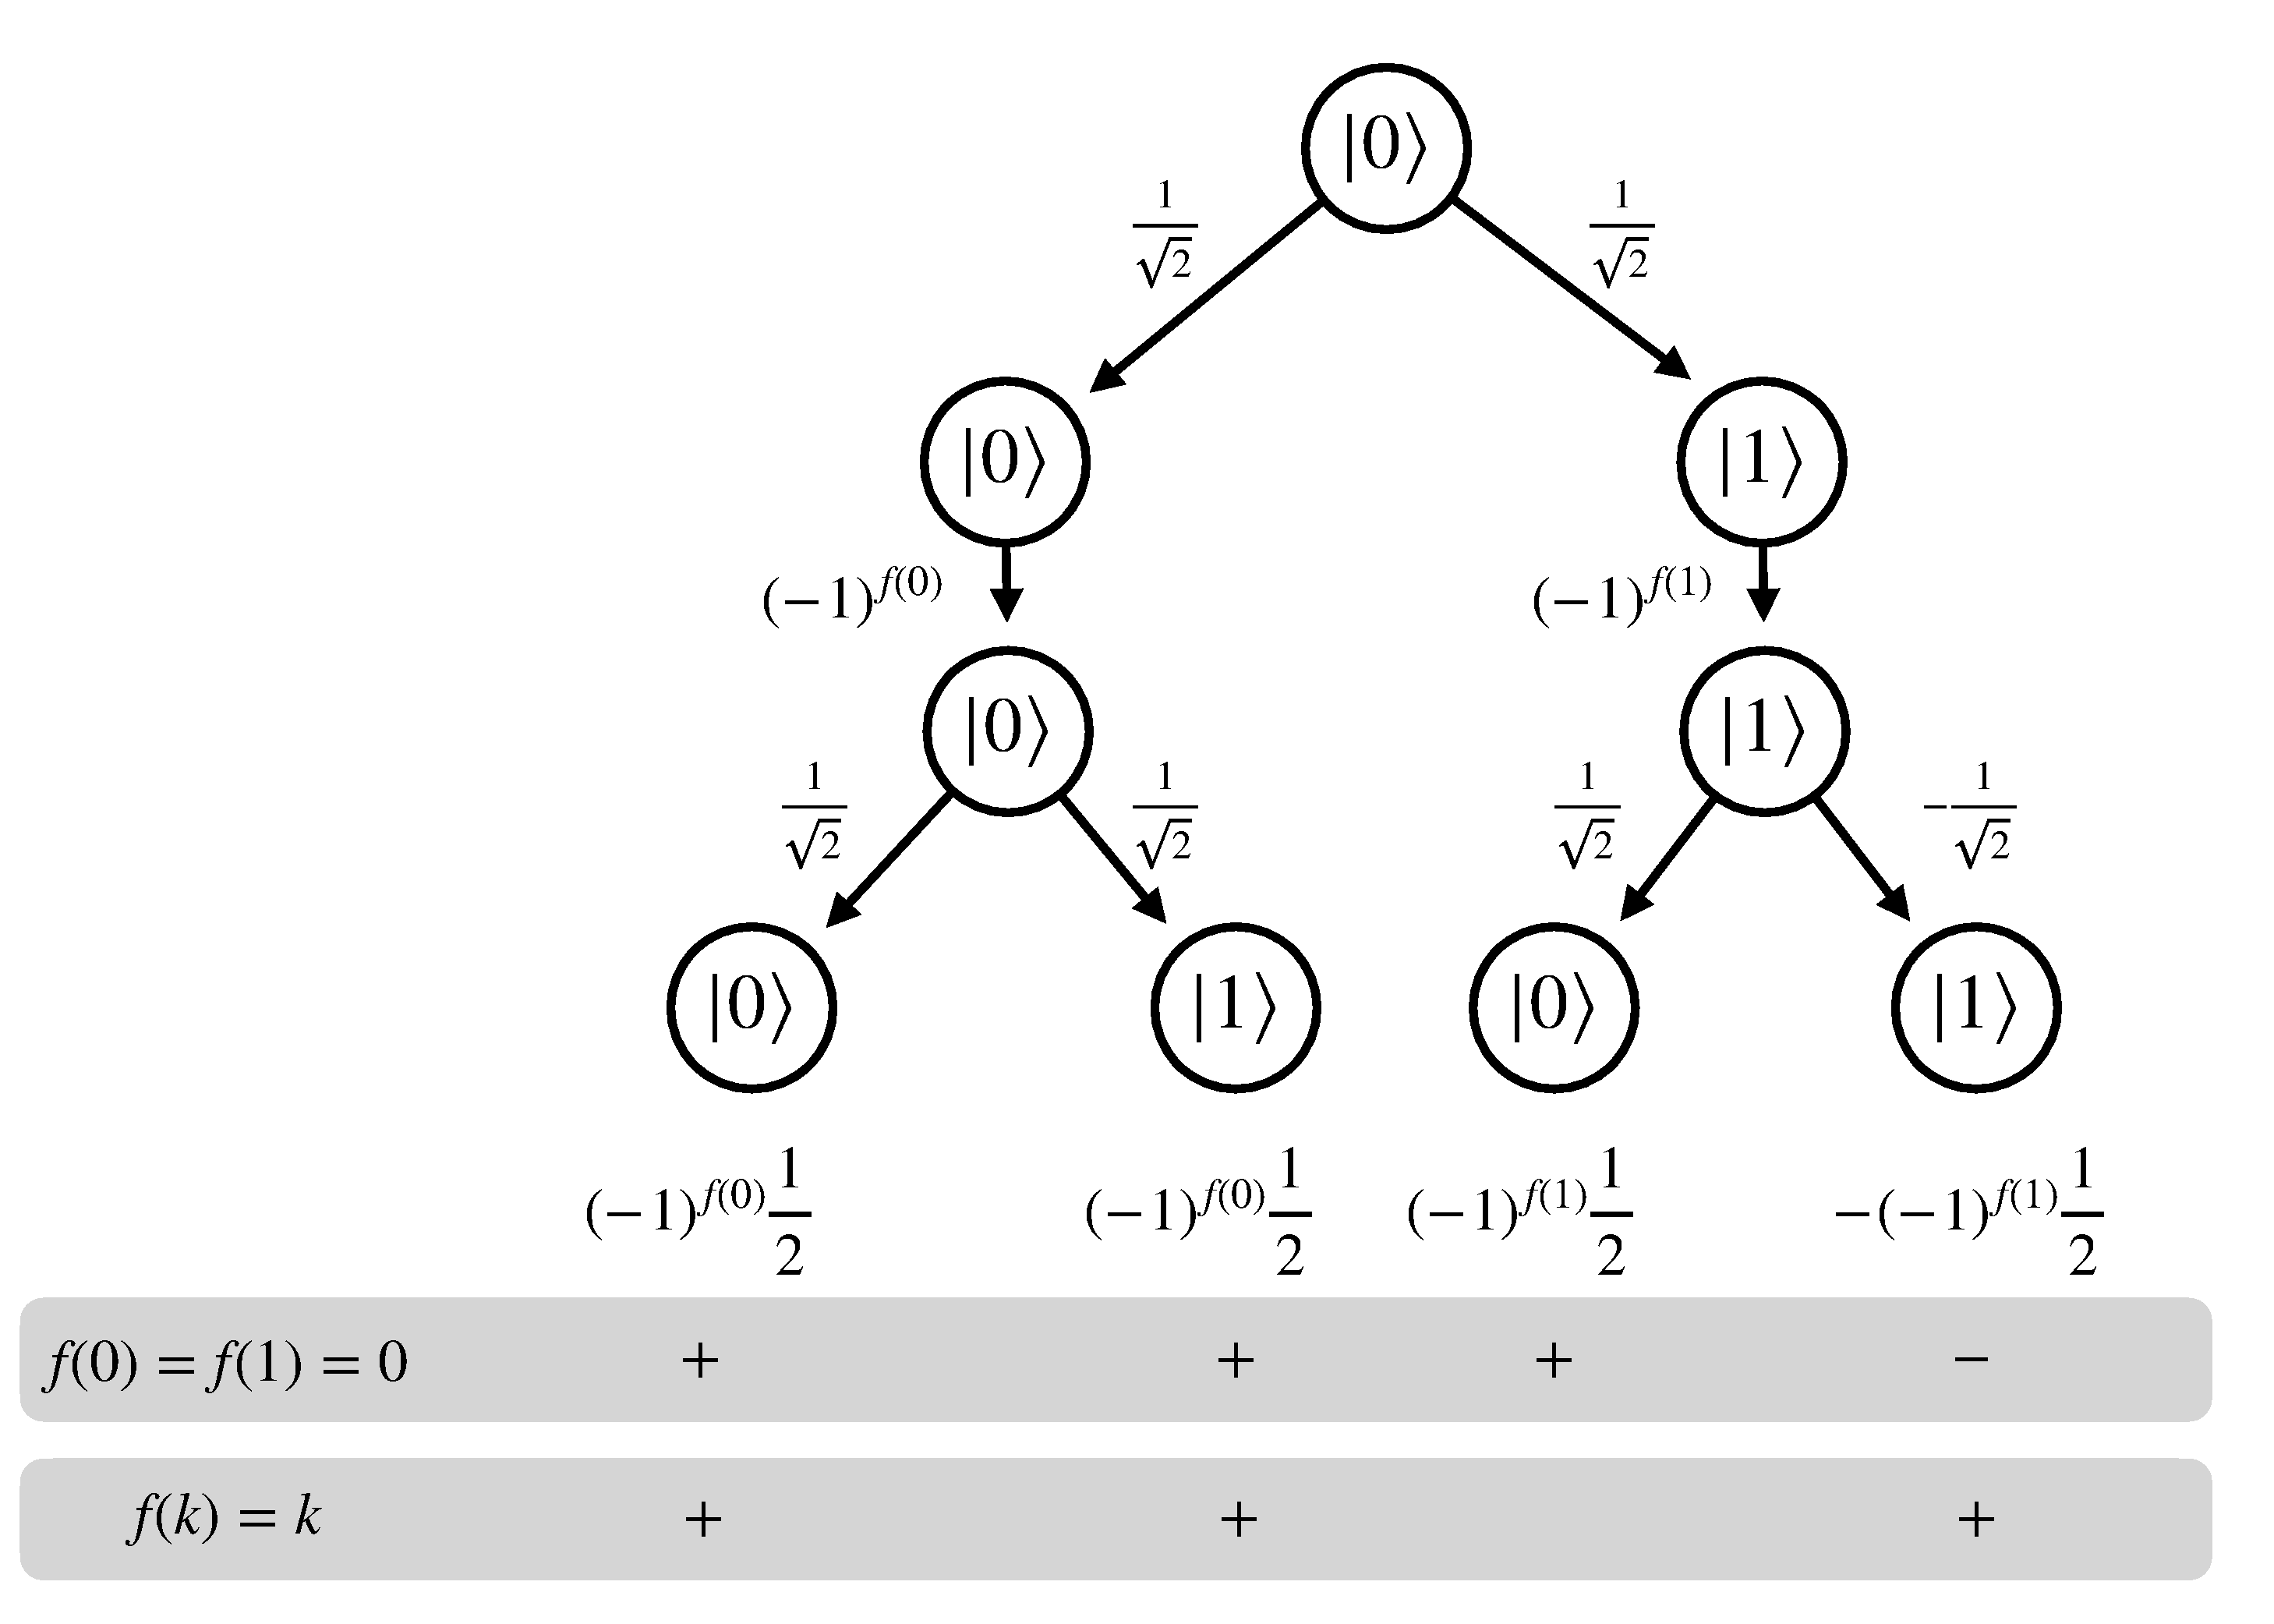
\includegraphics[width=0.75\textwidth]{src/deutsch-phase-oracle.pdf} 
\end{align*}
where we just indicate the signs of the amplitudes for two of the 4 possible $f$.



\subsection{Multi-Qubit Hadamard}
Before we start with the next example, it is useful to think about the action of Hadamard gates on multiple qubits.
A quantum state of multiple qubits can be written as a linear combination over all classical bit states (the ``computational basis states''). We can either label them as integers $\ket{\mathbf{k}}$ or by their explicit bit values $\ket{k_1k_2\dots k_N}$. Example for a 3 qubit basis states: $\mathbf{0}=000, \mathbf{1} = 001, \mathbf{2}=010, \dots ,\mathbf{5} = 101, \dots$. 
Often it can be useful to use the symbol $\otimes$ as a separator to indicate the individual qubits. Take for example
\begin{align}
    \ket{1011} = \ket{1}\otimes\ket{011} = \ket{10}\otimes\ket{11} = \ket{1}\otimes\ket{0}\otimes\ket{1}\otimes\ket{1}.
\end{align}
We can do this in the same way for operations. Take for example a 3 qubit system where we want to act with the Hadamard operation on the second qubit, we can denote this either by indicating the qubit onto which the operation acts in parentheses or explicitly using the $\otimes$ symbol
\begin{align}
    \hd(2) = 1 \otimes \hd \otimes 1.
\end{align}
If we are acting with $N$ Hadamard operations on $N$ qubits respectively, we can also use the short-notation
\begin{align}
    \hd^{\otimes N} = \hd(1) \hd(2) \dots \hd(N) = \bigotimes_{k=1}^{N} \hd =  \hd \otimes \hd \otimes \dots \otimes \hd.
\end{align}
A graphical notation -- a quantum circuit -- would be\\

\begin{center}
    $\hd^{\otimes 3}$ = \begin{quantikz}
& \gate{H} &[1cm]&\\
& \gate{H} &[1cm]&\\
& \gate{H} &[1cm]&\\
\end{quantikz}
\end{center}


where the wires represent the qubits and the boxes the operations. Note that quantum circuits are read from left to right.

In the same way, we can write for states
\begin{align}
    \ket{\mathbf{0}} = \ket{0}^{\otimes N} = \bigotimes_{k=1}^{N}\ket{0} = \ket{00\dots 0}
\end{align}
These are just different notations for the same thing. Depending on the context their usefulness will change.
Take for example $\hd \otimes \hd$, we know that this is a two-qubit operation, where a Hadamard operations will act on each qubit. In cases where we don't need explicit labels, this is convenient notation. If we need explicit labels, e.g. a Hadamard acting on qubit 3 and one on qubit 5 in a set of $N$ qubits, then $\hd(3) \hd(5)$ is more compact than $1\otimes 1 \otimes \hd \otimes 1 \otimes \hd \otimes 1 \otimes \dots \otimes 1 $
Now we can start to think about the action of such a collection of Hadmard gates on $N$ qubits.\\

Take $N$ qubits and let $N$ Hadamard gates act on each of them 
If acting on a $N$ bit basis state (a classical state corresponding to all $N$ bits being in either 0 or 1) we get
\begin{align}
    \hd^{\otimes N} \ket{k_1k_2\dots k_N} &=  \bigotimes_{i=1}^{N} \hd\ket{k_i} \nonumber\\ &= \bigotimes_{i=1}^{N} \frac{1}{\sqrt{2}}\left(\ket{0} + \left(-1\right)^{k_i} \ket{1} \right) \nonumber\\&=\frac{1}{\sqrt{2^N}} \sum_{l=0}^{2^N-1} \left(-1\right)^{\left(\sum_{i=1}^N k_il_i\right)} \ket{l_1 l_2\dots l_N}
\end{align}
If we introduce the shortcut 
\begin{def*}[bitwise dot-product]
\begin{align}
    \mathbf{l} \odot \mathbf{k} = l_1 k_1 \oplus l_2k_2 \oplus \dots \oplus l_N k_N
\end{align}
\end{def*}
for the bitwise dot-product between the $N$-bit binary representation of two integers $l$ and $k$, we can write
\begin{def*}[Hadamard basis]
\begin{align}
    H^{\otimes N} \ket{\mathbf{k}} = \frac{1}{\sqrt{2^N}} \sum_{\mathbf{l}=0}^{2^N-1} \left(-1\right)^{\mathbf{k}\odot \mathbf{l}} \ket{\mathbf{l}}.
\end{align}
\end{def*}
It is useful to verify this formula for yourself (ideally after you have gained some experience with these types of calculations), but for now, it is also fine to just use it.\\
Three important observations that we need later
\begin{highlight}
\begin{enumerate}
    \item if $\mathbf{k}=\mathbf{0}$ then all negative signs vanish from the right-hand-side.
    \item if $\mathbf{k}\neq\mathbf{0}$ then there will always be negative signs on the right-hand-side. On closer inspection: half of the $2^N$ basis states will get a negative sign.
    \item the states on the right-hand-side will be transformed into computational basis states when we act with a sequence of Hadamard operations on them (since Hadamards are self-inverse)
\end{enumerate}
\end{highlight}
\subsection{Deutsch-Jozsa}
A straightforward extension of the \texttt{Deutsch} algorithm is the algorithm by Deutsch and Jozsa. 
It has the same premise, but will lead to a (formal) exponential separation between classical and quantum realizations (again with respect to the number of queries to either the classical function $f$ or the quantum operation encoding $f$).\\
Starting from the Deutsch Problem that was asking if a Boolean function on a single bit is constant, we can go one step further and consider Boolean functions $f$ of $N$ bits. 
Here we will now ask if the function $f$ is constant ($\forall k: f(k) = x$ with constant $x\in\left\{0,1\right\}$ and $k$ being one of the $2^N$ possible assignments of the $N$ bits) or \textit{balanced}. The second states that for exactly half of the possible input bitstrings the function will evaluate to 0 and for the other half to 1. We can view this as a so-called ``promise Problem'', we ask if the function is constant, but we have the promise that the function is either constant of balanced.

\begin{def*}
\textbf{Deutsch-Jozsa Problem:} Given an $N$ bit Boolean function promised to be either constant or balanced, determine if its constant.
\end{def*}

\begin{algo*}
\textbf{Classical Algorithm:} We evaluate the function on $2^N/2+1$ different input states. If they all result in the same output, the function is constant, otherwise it's balanced (this is the promise). This has an exponential runtime in the number of calls to $f$.
\end{algo*}

\begin{algo*}[\texttt{Deutsch-Jozsa}]
As before, the algorithm is a bit more complicated, but a single call to $U_f$ will suffice!
The quantum operation is constructed similar to $U_\text{D}$ from \texttt{Deutsch}
\begin{align}
    U_\text{DJ} = \hd^{\otimes N} U_f \hd^{\otimes N} 
\end{align}
with the oracle $U_f$ acting as
\begin{align}
    U_f \ket{\mathbf{k}} = (-1)^{f(\mathbf{k})}\ket{\mathbf{k}}.
\end{align}
The algorithm applies $U_{\text{DJ}}$ on $N$ input qubits, all initialized to the $\ket{0}$ state
\begin{align}
         {U}_\text{DJ} \ket{\boldsymbol{0}} &= \begin{cases}
         \pm \ket{\mathbf{0}}, & f \text{ is constant}\\
         \pm \ket{\mathbf{k}}, \mathbf{k}\neq \mathbf{0} & f \text{ is balanced}
     \end{cases}
\end{align}
A single query to $U_f$ (contained in $U_\text{DJ})$ is sufficient to solve the problem.
\end{algo*}
As a quantum circuit, \texttt{Deutsch-Jozsa} (here for $N=3$) takes the form
\begin{center}
$ U_\text{DJ}$ = \begin{quantikz}
& \gate{H} & \gate[3]{U_f}& \gate{H} \\
& \gate{H} &[1cm] & \gate{H}\\
& \gate{H} &[1cm] & \gate{H}\\
\end{quantikz}
\end{center}
 Acting on $N$ qubits in the zero state we have
 \begin{align}
      {U}_\text{DJ} \ket{0}^{\otimes N} &= \frac{1}{\sqrt{2^N}} \hd^{\otimes N}\sum_{k=0}^{2^N-1} {U}_f \ket{\mathbf{k}}\nonumber \\
      &= \frac{1}{\sqrt{2^N}} \hd^{\otimes N}\sum_{k=0}^{2^N-1} (-1)^{f(\mathbf{k})}\ket{\mathbf{k}}.
 \end{align}
 If $f(\mathbf{k})$ is constant, either have $f\mathbf{(k)}=1$ or $f({\mathbf{k}})=0$ in all case this will, after application of the remaining Hadamard operation (see observation 1 above), lead to either $\pm\ket{0}^{\otimes N}$ where the choice of $\pm$ will depend on the value that $f=const$ takes. The sign has however no impact on the probability to read out the state $\ket{0}^{\otimes N}$ (all qubits in state $\ket{0}$) which is 100\% in this case.
 If $f$ is balanced on the other hand, then half of the signs will be negative, which will lead to a basis state $\ket{\mathbf{k}}$ with $\mathbf{k}\neq 0$ after the final Hadamard operations are applied (see observation 2 above).\\
 In summary we arrive at
 \begin{align}
     {U}_\text{DJ} \ket{0}^{\otimes N} &= \begin{cases}
         \pm \ket{\mathbf{0}}, & f \text{ is constant}\\
         \pm \ket{\mathbf{k}}, \mathbf{k}\neq \mathbf{0} & f \text{ is balanced}
     \end{cases}
 \end{align}

 \paragraph{Exponential Speedup:} \texttt{Deutsch-Jozsa}  has an exponential speedup when we compare the quantum algorithm: only a \textit{single} query to $U_f$ is necessary, while classically we require $2^N/2 + 1$ queries to $f$. These are exponentially more queries in the classical counterpart.\\
On a second look we do however realize that this exponential speedup only holds if we compare with a deterministic classical strategy with 100\% certainty. We can ask ourselves: What if, we only sample $M$ of the possible $2^N$ inputs to $f$. Assume for now that $f$ is not constant, we evaluate $f$ on one of the possible inputs (let's say $f(0000...0)=x$), you can call this a ``gauge query'' because now we need only ask for each new query if it will reach the same value $x$. With each sample of the possible inputs we have a 50\% chance to get an input $k$ that leads to $f(k)\neq x$, at this point, we know for sure that $f$ is not constant. The chances of sampling a $k$ with this property are always $1/2$, so on average we will arrive at $2$ queries~\footnote{details not important here; see info3 lecture on average case analysis. This example is basically the same} to $f$ in order to determine that $f$ is not constant (in total we have then 3 queries, counting the gauge query as well). In the case where $f$ is constant, the argument is the same, just with insecurity about the current assumption that $f$ is constant.
All in all, the speed-up shrinks basically down to the original Speedup of a factor of 2 (plus one gauge query). 

\subsection{Bernstein-Vazirani}
A slight modification of Deutsch-Jozsa leads to the \texttt{Bernstein-Vazirani} algorithm. Here we can show a polynomial improvement (from linear to constant) in the number of queries when comparing the quantum algorithm with the best possible classical algorithm. 

\begin{def*}[Bernstein-Vazirani problem]
    Given is a Boolean function $f$ acting on $N$ bits with the promise that $f(\mathbf{x}) = \mathbf{x}\odot \mathbf{y} =  x_1y_1 \oplus x_2y_2 \oplus \dots \oplus x_Ny_N$ (bit wise binary dot-product) with an unknown $N$-bit string $\mathbf{y}$. The task is to find $\mathbf{y}$.
\end{def*}

\begin{algo*}[Classical solution]
    Classically we can query $f$ with the $N$ ``unary'' bitstrings $\mathbf{x}_1 = 000\dots 01, \mathbf{x}_2 = 000\dots 10, \dots, \mathbf{x}_N = 100\dots 00$. Each query will reveal one bit of $\mathbf{y}$ via $f(\mathbf{x}_i) = \mathbf{x}_i \odot\mathbf{y} = y_i$. So we need exactly $N$ queries to determine $\mathbf{y}$ and we can not get away with less.
\end{algo*}

\begin{algo*}[\texttt{Bernstein-Vazirani}]
We perform the \texttt{Deutsch-Jozsa} operation where $U_f$ encodes the $f$ from the Bernstein-Vazirani problem to the all-zero state
    \begin{align}
         {U}_\text{DJ} \ket{\mathbf{0}} &= \ket{\mathbf{y}}
\end{align}
the resulting state is the sought bitstring $\mathbf{y}$ which can now just be read-out from the qubit register.  
We just need a single query to $U_f$ to get the answer with 100\%.
\end{algo*}
To see that this is actually true:
\begin{align}
U_\text{DJ}\ket{\mathbf{0}} &= \hd^{\otimes N} U_f \hd^{\otimes N}\ket{\mathbf{0}} \nonumber\\
&= \hd^{\otimes N} \frac{1}{\sqrt{2^N}} \sum_{k=0}^{2^N-1} U_f\ket{\mathbf{k}} \nonumber\\
&= \hd^{\otimes N} \frac{1}{\sqrt{2^N}} \sum_{k=0}^{2^N-1} (-1)^{\mathbf{k}\odot \mathbf{y}}\ket{\mathbf{k}}\nonumber\\
&= \ket{\mathbf{y}}
\end{align}
Where we have used observation 3 from above in the last step. Note that the only thing that changed w.r.t to \texttt{Deutsch-Jozsa}  is the promise on $f$.\\

The polynomial separation that we are seeing here between classical and quantum is not bad, but it can actually be improved to achieve an exponential separation w.r.t queries to $U_f$ and $f$ for specifically constructed decision problems within BQP (the quantum analog of P) and BPP (the probabilistic analog of P). We will skip the details here.
\clearpage

\subsection{Summary}
First encounters with key concepts in quantum information processing:
\begin{itemize}
    \item wavefunctions
    \item interference
    \item linear operators 
    \item probability amplitudes
    \item qubits
    \item the \textsc{hadamard} operation
    \item path sum representations
\end{itemize}


We have also seen examples of quantum Algorithms that have advantages over classical algorithms with respect to query complexity
\begin{enumerate}
    \item \texttt{Deutsch}: single query (quantum) vs two queries (classical)
    \item \texttt{Deutsch-Jozsa}: single query (quantum) vs $\Theta(2^N)$ queries (cassical) -- if we tolerate small errors we will however get away with $3$ queries on average.
    \item \texttt{Bernstein-Vazirani}: single query (quantum) vs $N$ queries (classical)
\end{enumerate}

We also observe here that the proven speedups are only with respect to query complexity. Meaning that the ``oracle'' $U_f$ is already given to you. With the exception of the plain \texttt{Deutsch} algorithm, the speedup also just works because we are given a promise (constant or balanced, or the promise that the Boolean function has a specific structure).\\


